\section{Trigger and event Selection}

\subsection{Trigger selection}
\label{sec:DiHiggs:trigger}

The ATLAS trigger system, as described in section~\ref{sec:ATLAS:trigger},
consists of the hardware-based level (L1) and the software-based level (HLT)
to select characteristic events. 
Events in the \lephad\ channel
are recorded using a combination of single-lepton triggers (SLTs) 
and lepton-plus-\tauhad\ triggers (LTTs). 
The offline objects are required to pass addition 
\pt\ cuts. For the leptons($e$ or $mu$), a threshold which is
1~GeV higher than the HLT \pt\ threshold is applied to
reach its efficiency plateau region. 
For the \tauhad, the threshold is set at 5~GeV above the
HLT \pt\ requirement for the same reason.
The offline $e$, $mu$ and \tauhad\ must be matched to
the corresponding trigger objects. 

The priority is given to SLT events if a lepton fufils
the offline lepton \pt\ requirements. 
A combination of various un-prescaled 
\footnote{The trigger rate is reduced by \textit{prescaling} which randomly 
vetos events that pass the trigger.} 
single electron triggers (SET) 
and single muon triggers (MET) are used to 
maximise the efficiency.
As the \pt\ threshold is raised for 1~GeV for the 
HLT \pt\ requirements,
the single electron triggers (SET) 
require an event with an electron with \pT > 25 or > 27~\GeV,
whereas the single muon triggers (SMT) require an event with a 
muon with \pT > 21 or > 27~\GeV,  depending on the data-taking period.

The SLT triggers used are listed in Table~\ref{tab:SLTtriggers_lephad}. 
In this table, the following naming conventions are used:
the trigger names begin with HLT, followed by the 
lepton type (e or mu for an electron or muon respectively) and the 
HLT \pt\ threshold. 
What comes next is the identification WP (loose, medium or tight), 
prefixed with `lh'which stands for likelihood-based trigger. 
The suffix of `nod0' indicates that no impact parameter cuts are
applied. 
For SMT, no identification is applied 
therefore it is not specified. 
The following is the isolation requirement, 
specified by `i' and the working point (varloose, varmedium).
If not specified, no isolation requirement is applied.
Finally, the suffix which starts `L1EM' (`L1MU') indicates the 
object is seeded with L1 electromagnetic (muonic) trigger items, 
with \pt\ threshold specified by the number after; the `VH' stands for 
the \pt\ threshold varies with eta to account for energy loss
and hadronic core isolation is applied. If not specified,
the L1 seed is using the default setting. 


\begin{table}
        % \centering
  \scriptsize
  \begin{tabular}{lll}
  %  \toprule
    %Trigger & Period \\
    \midrule
    \multicolumn{3}{c}{\textbf{Single Lepton Triggers (SLT)}} \\
    \midrule
    \textbf{Period} & \textbf{Single Electron Triggers (SET)} 
    & \textbf{Single Muon Triggers (SMT)}   \\
    \midrule 
    \multirow{3}{*}{2015} & HLT\_e24\_lhmedium\_L1EM20VH &HLT\_mu20\_iloose\_L1MU15\\
    & HLT\_e60\_lhmedium  & HLT\_mu50  \\
    & HLT\_e120\_lhloose & \\
    \midrule
    \multirow{3}{*}{2016 \& 2017 \& 2018} & HLT\_e26\_lhtight\_nod0\_ivarloose  & HLT\_mu26\_ivarmedium \\
    & HLT\_e60\_lhmedium\_nod0  & HLT\_mu50\\
    & HLT\_e140\_lhloose\_nod0 \\
 \bottomrule
  \end{tabular}
 \caption{SLT triggers used in the \lephad channel, along with the trigger-dependent offline \pT\ thresholds, for each year/period are shown.
 Table reproduced from internal notes of the analysis.}
  \label{tab:SLTtriggers_lephad}
\end{table}


The LTT triggers used are listed in Table~\ref{tab:SLTtriggers_lephad}. 
For the LTT triggers, an electron (muon) is required with
\pt\ > 18 (15)~GeV, together with 
a \tauhad\ with \pt\ > 30~GeV or 40~GeV depending on the period.
Jets are cut at 80~GeV (45~GeV) for Level-1 trigger \pt-thresholds of 25~GeV (12~GeV)
(the L1 jets \pt\ requirements are explained in the following). 
The same naming conventions are used for the LTT triggers. 
In addition, the trigger names are expanded by the `tau' which 
stands for \tauhad\ followed by its \pt, identification requirements
and pre-selection settings. Again, unless specified, the default
L1 seeds are used. For dedicated L1 seeds, the lepton (`EM' for electron
or MU for muon) followed by \pt\ requirements and specific settings. 
After the lepton, the number of \tauhad\ is specified by a number before 
`TAU', followed by a number indicating the \pt\ threshold. For example, 
`2TAU12I' stands for two \tauhad\ with \pt\ > 12, with electromagnetic
isolation applied (`I'). Finally, the number of jets and the \pt\ requirements
are specified in the same fashion. If unspecified, at least one jets with \pt\ > 25~GeV
are required (the offline cut is raised to 80~GeV).

\begin{table}[h]
    \centering
   \scriptsize
    \begin{tabular}{l}
    %  \toprule
      %Trigger & Period \\
      \midrule
      \multicolumn{1}{c}{\textbf{Lepton Tau Triggers (LTT)}} \\
      \midrule
      \textbf{Electron Tau Triggers (ETT)}   \\
      \midrule
         HLT\_e17\_lhmedium\_nod0\_tau25\_medium1\_tracktwo \\	
         HLT\_e17\_lhmedium\_nod0\_ivarloose\_tau25\_medium1\_tracktwo \\
         HLT\_e17\_lhmedium\_nod0\_ivarloose\_tau25\_medium1\_tracktwo\_L1EM15VHI\_2TAU12IM\_4J12  \\
         HLT\_e17\_lhmedium\_nod0\_ivarloose\_tau25\_medium1\_tracktwoEF \\
         HLT\_e17\_lhmedium\_nod0\_ivarloose\_tau25\_medium1\_tracktwoEF\_L1EM15VHI\_2TAU12IM\_4J12 \\
         HLT\_e17\_lhmedium\_nod0\_ivarloose\_tau25\_mediumRNN\_tracktwoMVA  \\
         HLT\_e17\_lhmedium\_nod0\_ivarloose\_tau25\_mediumRNN\_tracktwoMVA\_L1EM15VHI\_2TAU12IM\_4J12 \\
     \midrule
     \textbf{Muon Tau Triggers (MTT)} \\
       \midrule
         HLT\_mu14\_tau25\_medium1\_tracktwo  \\		
         HLT\_mu14\_ivarloose\_tau25\_medium1\_tracktwo  \\
         HLT\_mu14\_ivarloose\_tau25\_medium1\_tracktwo\_L1MU10\_TAU12IM\_3J12   \\	
         HLT\_mu14\_ivarloose\_tau25\_medium1\_tracktwoEF\_L1MU10\_TAU12IM\_3J12  \\
         HLT\_mu14\_ivarloose\_tau25\_mediumRNN\_tracktwoMVA\_L1MU10\_TAU12IM\_3J12 \\	
         HLT\_mu14\_ivarloose\_tau35\_medium1\_tracktwo   \\	
         HLT\_mu14\_ivarloose\_tau35\_medium1\_tracktwoEF  \\
         HLT\_mu14\_ivarloose\_tau35\_mediumRNN\_tracktwoMVA\\
      \bottomrule
    \end{tabular}
    \caption{LTT triggers used in the \lephad\ channel. For different periods, 
    a mixture of triggers from this list are used. Table reproduced from analysis internal notes.  }
    \label{tab:LTT_trigger_names}
  \end{table}

\subsection{Event pre-selection}

\label{sec:DiHiggs:selection}



Before passing the events to the MVA algorithm, 
they are required to pass a loose pre-selection criteria to 
select events consistent with the signal topology and to
remove obvious background.  
Events passing the pre-selection criteria is referred to as
signal region (SR) events. 
Events are required to contain exactly 
one electron or muon, 
an oppositely charged \tauhad\, 
and exactly two $b$-tagged jets.
The selected electron (muon) must pass a 
tight (medium) identification requirement with an efficiency of around 80\% (97\%).
% and the (sub-)leading $b$-tagged jet is required to have \pt$>45~(20)$~GeV. 
If more than one primary vertex is present in the events, 
the one with the highest $(p_T^{track})^2$ is chosen.
To reject background events from low-mass Drell-Yan events, 
the invariant mass of the $\tau$-lepton pair ($m_{\tau\tau}^\text{MMC}$),
is required to be above 60~GeV,
which is estimated from the four-momenta of the electron or muon, 
the \tauhad\ and the \met\ using the Missing Mass Calculator (MMC)~\cite{Elagin:2010aw}.
In the calculation, the \met\ is assumed to be exclusively from the neutrinos 
produced in the $\tau$-lepton decays. 
To reject the \ttbar\ events, the $b$-tagged jet pair invariant mass ($m_{bb}$) 
is required to be less than 150~GeV. And therefore, by reversing this cut, 
a $t\bar t$-enriched region can be defined  
which is used in the estimation of $t\bar t$ backgrounds
as described in Section~\ref{sec:DiHiggs:lephadfake}. 
A \tauhad\ with $\pt>20$~GeV and 
$\vert\eta\vert<2.3$ is required in the SLT category.
A \tauhad\ with $\pt>30$~GeV,
or higher if required by the by the LTT triggers (as defined in the previous
section~\ref{sec:DiHiggs:trigger}), 
and $\vert\eta\vert<2.3$ is required in the LTT events. 
In both categories, the (sub-)leading $b$-tagged jet 
must have $\tau_pt>45~(20)$~GeV, 
in addition to any trigger-dependent jet requirements of LTT
defined in the previous section.
The full event pre-selection is summarised in Table~\ref{tab:DiHiggs:selectionsummary}. 

\begin{table}[htbp]
    \centering
    \resizebox{0.72\textwidth}{!}{
    \begin{tabular}{C{0.39\textwidth}C{0.39\textwidth}}
    \toprule
    \multicolumn{2}{c}{$\tau_\text{lep}\tau_\text{had}$ categories}\\
    %% Single-$\tau_\text{had}$ trigger (STT) & Di-$\tau_\text{had}$ trigger (DTT) & Single-$e/\mu$ trigger (SLT) & $e/\mu+\tau_\text{had}$ trigger (LTT)\\
    SLT & LTT\\
    \midrule
    \multicolumn{2}{c}{\BF{$e/\mu$ selection}}\\
    \multicolumn{2}{c}{Exactly one tight $e$ or medium $\mu$}\\
    $p_\text{T}^e>25,27~\text{GeV}$ & $18~\text{GeV}<p_\text{T}^e<\text{SLT cut}$\\
    $p_\text{T}^\mu>21,27~\text{GeV}$ & $15~\text{GeV}<p_\text{T}^\mu<\text{SLT cut}$\\
    \multicolumn{2}{c}{$\vert\eta^e\vert<2.47$, not $1.37<\vert\eta^e\vert<1.52$}\\
    \multicolumn{2}{c}{$\vert\eta^\mu\vert<2.7$}\\
    \midrule
    \multicolumn{2}{c}{\BF{\tauhad\ selection}}\\
    \multicolumn{2}{c}{One loose \tauhad}\\
    \multicolumn{2}{c}{$\vert\eta\vert<2.3$}\\
   \pt$>20~\text{GeV}$ & \pt$>30~\text{GeV}$\\
    \midrule
    \multicolumn{2}{c}{\BF{Jet selection}}\\
    \multicolumn{2}{c}{$\geq 2$ jets with $\vert\eta\vert<2.5$}\\
    \pt$>45~(20)~\text{GeV}$ & Trigger dependent\\
    \midrule
    \multicolumn{2}{c}{\BF{Event-level selection}}\\
    \multicolumn{2}{c}{Trigger requirements passed}\\
    \multicolumn{2}{c}{Collision vertex reconstructed}\\
    \multicolumn{2}{c}{$m_{\tau\tau}^\text{MMC}>60~\text{GeV}$}\\
    \multicolumn{2}{c}{Opposite-sign electric charges of $e/\mu/\tau_\text{had-vis}$ and \tauhad}\\
    \multicolumn{2}{c}{Exactly two $b$-tagged jets}\\
    %% \multicolumn{4}{c}{$b$-tagged jet \pt$>45~(20)~\text{GeV}$}\\
   \multicolumn{2}{c}{$m_{bb}<150~\text{GeV}$}\\
    \bottomrule
    \end{tabular}
    }
    \caption{Summary of the event preselections, 
    shown separately for the SLT and LTT. 
   Thresholds on the (sub-)leading \pt\ object are given 
   outside (within) parentheses. 
   The possible values of the requirements in the SLT are separated by commas
   which depends on the year of the data-taking. 
   For the jet selection in the LTT channel multiple selection criteria are used.
   %  as described 
   % in Section~\ref{sec:DiHiggs:triggers}. 
   The trigger \pt\ thresholds shown correspond to the offline requirements.
   Table reproduced from Ref.~\cite{dihiggs-conf}.}
   \label{tab:DiHiggs:selectionsummary}
\end{table}


The rate of events accepted by the detector is quantified by the \textit{acceptance},
and the rate of events selected by the analysis selection is quantified by 
the \textit{selection efficiency}.
These two rates are usually multiplied together ($A \times \epsilon$) to quantify the rate of a simulated event
accepted by the detector and the analysis selection. 
The cumulative $A \times \epsilon$ in each step of the pre-selection
is summarised in Table~\ref{tab:DiHiggs:cutflowslt}
and Table~\ref{tab:DiHiggs:cutflowltt}
for the SLT and LTT channels, respectively, for the
non-resonant signal and three example resonances mass points.  


\begin{table}[!htbp]
    \centering
    
    \resizebox{0.92\textwidth}{!}{
      \begin{tabular}{lccccc}
        \toprule
                  &       \multicolumn{2}{c}{Non-resonant signal}     & \multicolumn{3}{c}{Resonant signal} \\ \cline{4-6}
        Selection & ggF $HH$ & VBF $HH$ & (300~GeV) & (500~GeV) & (1000~GeV) \\
        \midrule
        Basic selection     &  19\%  &  16\%  &  13\%  &  22\%  &  30\% \\
        Trigger           &  12\%  &  9.2\%  &  6.0\%  &  14\%  &  22\% \\
        Object selections &  9.7\%  &  7.2\%  &  5.0\%  &  11\%  &  20\% \\
        Trigger specific offline $p_\text{T}$ cuts 
                          &  9.5\%  &  6.8\%  &  4.4\%  &  11\%  &  20\% \\
        Opposite-charged $\tau$ and lepton
                          &  9.4\%  &  6.6\%  &  4.4\%  &  11\%  &  20\% \\
        Two $b$-tagged jets
                          &  4.4\%  &  2.7\%  &  1.8\%  &  4.9\%  &  10\% \\
       $m^\text{MMC}_{\tau\tau}>60~\text{GeV}$ 
                          &  4.3\%  &  2.7\%  &  1.8\%  &  4.8\%  &  9.7\% \\
        $m_{bb}<150~\text{GeV}$ 
                          &  4.1\%  &  2.6\%  &  1.7\%  &  4.6\%  &  9.2\% \\
        \bottomrule
      \end{tabular}
    }
\large
\caption{Cumulative $A \times \epsilon$ for simulated signal events to pass each stage of the event pre-selection in the SLT channel. 
The efficiencies are calculated with respect to $HH\to b\bar b\tau^+\tau^-$ decays in which one $\tau$-lepton decays hadronically and one decays leptonically.
The `Basic selection' includes selections with at least one \tauhad\ candidate and one lepton passing loose kinematic requirements.
The `Object selections' requires exactly one \tauhad\ candidate, at least two jets with $p_\text{T}>25$ GeV and $\vert\eta\vert < 2.5$.
The `Trigger specific offline $p_\text{T}$ cuts' are cuts placed on the $p_\text{T}$ of the reconstructed jet or \tauhad\
that are geometrically matched to the HLT objects, to ensure the efficiencies of the HLT objects reach the plateau region.
}
\label{tab:DiHiggs:cutflowslt}
\end{table}
    

\begin{table}[!htbp]
    \centering
    
    \resizebox{0.92\textwidth}{!}{
    \begin{tabular}{lccccc}
    \toprule
    &       \multicolumn{2}{c}{Non-resonant signal}     & \multicolumn{3}{c}{Resonant signal} \\ \cline{4-6}
    Selection & ggF $HH$ & VBF $HH$ & (300~GeV) & (500~GeV) & (1000~GeV) \\
    \midrule
    Basic selection     &  19\%  &  16\%  &  13\%  &  22\%  &  30\% \\
    Trigger           &  3.4\%  &  3.2\%  &  2.8\%  &  4.0\%  &  3.4\% \\
    Object selections &  2.9\%  &  2.3\%  &  2.2\%  &  2.8\%  &  2.4\% \\
    Trigger specific offline $p_\text{T}$ cuts 
                        &  2.3\%  &  1.8\%  &  1.4\%  &  2.6\%  &  2.3\% \\
    Opposite-charged $\tau$ and lepton
                        &  2.3\%  &  1.8\%  &  1.4\%  &  2.6\%  &  2.3\% \\
    Two $b$-tagged jets
                        &  1.1\%  &  0.76\% &  0.61\% &  1.2\%  &  1.1\% \\
    $m^\text{MMC}_{\tau\tau}>60~\text{GeV}$ 
                        &  1.0\%  &  0.75\% &  0.61\% &  1.2\%  &  1.1\% \\
    $m_{bb}<150~\text{GeV}$ 
%%%                      &  0.985\% &  0.709\% &  0.569\% &  1.11\%  &  1.02\% \\
                        &  0.98\%  &  0.71\%  &  0.57\%  &  1.1\%  &  1.0\% \\
    \bottomrule
    \end{tabular}
    }
    \large
\caption{Cumulative $A \times \epsilon$ for simulated signal events to pass each stage of the event pre-selection in the LTT channel. 
The efficiencies are calculated with respect to $HH\to b\bar b\tau^+\tau^-$ decays in which one $\tau$-lepton decays hadronically and one decays leptonically. 
The `Basic selection' includes selections with at least one \tauhad\ candidate and one lepton passing loose kinematic requirements.
The `Object selections' requires exactly one \tauhad\ candidate, at least two jets with $p_\text{T}>25$ GeV and $\vert\eta\vert < 2.5$.
The `Trigger specific offline $p_\text{T}$ cuts' are cuts placed on the $p_\text{T}$ of the reconstructed jet or \tauhad\
that are geometrically matched to the HLT objects, to ensure the efficiencies of the HLT objects reach the plateau region.
}
\label{tab:DiHiggs:cutflowltt}
\end{table}


The $A \times \epsilon$ for all resonances mass points are shown 
in Figure~\ref{fig:selection:acceptances}. 
The decrease in $A \times \epsilon$ 
for $m_X$ greater than about 1000~GeV is due to the Lorentz boost 
of the Higgs bosons causing their decay products to become highly collimated more often.

\begin{figure}[htbp]
\centering
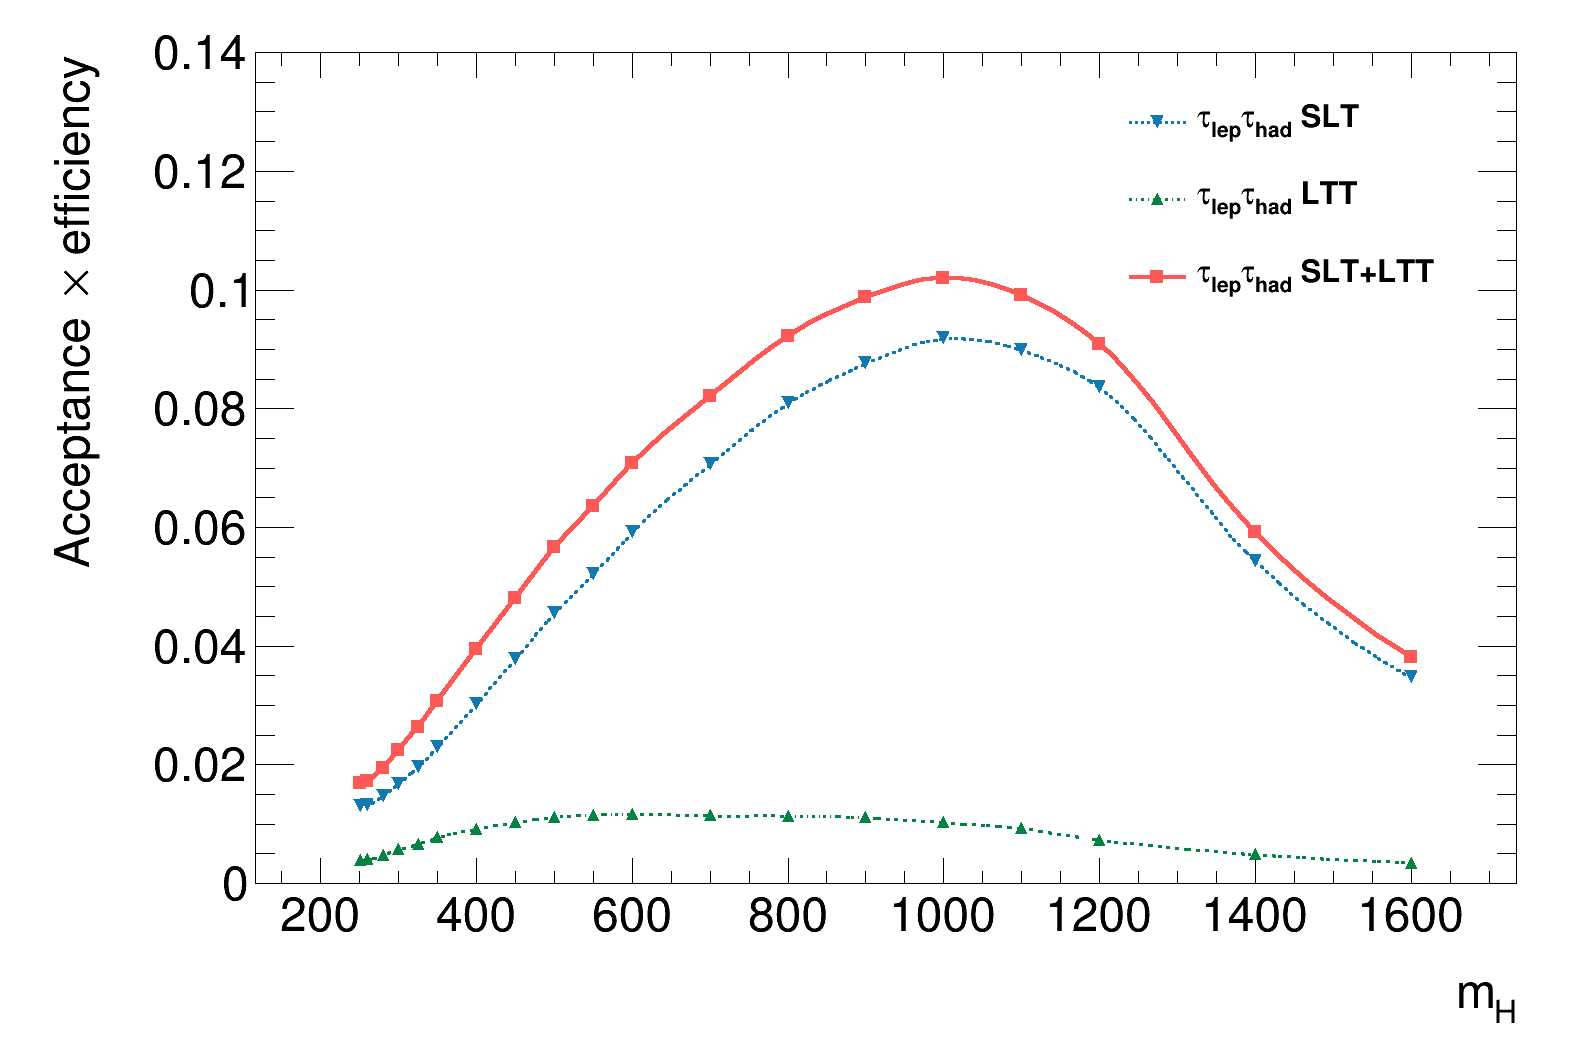
\includegraphics[width=0.85\linewidth]{DiHiggs/plots/FF_CRs/testacc.png}
% location:/hepstore/zhiyuan/Code_latest/test, run  python ../plotcasual.py to get
\caption{$A \times \epsilon$ for the resonant Di-Higgs production
as a function of the resonance mass $m_X$ in
SLT, LTT and SLT LTT combined.}
\label{fig:selection:acceptances}
\end{figure}

After the pre-selection, the event yields of the data,
signal and background and the corresponding
statistical error is shown in Table.~\ref{tab:tab:LepHadSLTYields} for the 
SLT channel, and Table.~\ref{tab:LepHadLTTYields} for the LTT channel.
The `Fake' background in the table represents the background due to a jet faking
a \tauhad, which is estimated by a
data-driven background described in details in section~\ref{sec:DiHiggs:lephadfake}.
\begin{table}
  \centering
  \scriptsize
  \begin{tabular}{|c|c|c|c|c|}
    \hline
\hline
SampleName & Entries & Integral & Error & Error/Integ.\\
\hline
\multicolumn{5}{|c|}{\textbf{Signal Samples}} \\
\hline
ggF Non-resonant      &151522 &5.872	 & 0.018&0.3\% \\ 
VBF Non-resonant	   	&36457  &  0.2002 &0.0013&0.6\% \\
Resonant at $m_X$ =251	& 22541 &	 60.6 &  0.4& 0.7\% \\
Resonant at $m_X$ =260	& 22252 &	60.9 &  0.4& 0.7\% \\
Resonant at $m_X$ =280	& 24595 &	 67.9 &  0.4& 0.7\% \\
Resonant at $m_X$ =300	& 18398 &	 77.2 &  0.6& 0.8\% \\
Resonant at $m_X$ =325	& 20904 &	90.9 &  0.6& 0.7\% \\
Resonant at $m_X$ =350	& 23593 &	 106.4 &  0.7& 0.7\% \\
Resonant at $m_X$ =400	& 29280 &	 140  +&  0.8& 0.6\% \\
Resonant at $m_X$ =450	& 34665 &	 175.3 &  1& 0.6\% \\
Resonant at $m_X$ =500	& 21332 &210.7 &  1.5& 0.7\% \\
Resonant at $m_X$ =550	& 23571 &240.9 &  1.6& 0.7\% \\
Resonant at $m_X$ =600	& 25917 &273.9 &  1.8& 0.6\% \\
Resonant at $m_X$ =700	& 29596 &327  +&  2& 0.6\% \\
Resonant at $m_X$ =800	& 32606 &74.5 &  2.1& 0.6\% \\
Resonant at $m_X$ =900	& 34392 &405.6 &  2.3& 0.6\% \\
Resonant at $m_X$ =1000	& 35119 &425.2 &  2.3& 0.6\% \\
Resonant at $m_X$ =1100	& 44157 &416.2 &  2& 0.5\% \\
Resonant at $m_X$ =1200	& 32337 &386.9 &  2.4& 0.6\% \\
Resonant at $m_X$ =1400	& 25539 &251.1 &  1.6& 0.7\% \\
Resonant at $m_X$ =1600	& 14421 &160.6 &  1.4& 0.9\% \\
\hline
\multicolumn{5}{|c|}{\textbf{Background Samples}} \\
\hline
Fake    &         2089776         &33920        &110           &       0.3\%      \\
ttbar     &         490058          &61620        &90           &       0.1\%      \\
stopWt    &         25910         &3054        &20           &       0.7\%      \\
stopt     &         5798          &596        &11           &       1.8\%      \\
stops     &         1450          &38.8        &1.1           &       2.8\%      \\
Zttbb     &         21473         &1426        &27           &       1.9\%      \\
Zttbc     &         1746          &132        &10           &       7.6\%      \\
Zttbl     &         1184          &63        &7           &       11.1\%      \\
Zttcc     &         608         &134        &22           &       16.4\%      \\
Zttcl     &         216         &13        &9           &       69.2\%      \\
Zttl    &         122         &16        &6           &       37.5\%      \\
Wtt     &         76          &5.4        &0.8           &       14.8\%      \\
W     &         747         &75        &8           &       10.7\%      \\
Zbb     &         17645         &796        &26           &       3.3\%      \\
Zbc     &         1467          &75        &9           &       12.0\%      \\
Zbl     &         1006          &39        &6           &       15.4\%      \\
Zcc     &         278         &79        &20           &       25.3\%      \\
Zcl     &         135         &22        &10           &       45.5\%      \\
Zl    &         30          &4.1        &2           &       48.8\%      \\
ZZ    &         6754          &82.8        &2           &       2.4\%      \\
WW    &         110         &13.3        &2.1           &       15.8\%      \\
WZ    &         1992          &58.5        &2.6           &       4.4\%      \\
ttH     &         133199          &92.99        &0.33           &       0.4\%      \\
VBFHtautau    &         933         &1.41        &0.05           &       3.5\%      \\
ggFHtautau    &         2159          &17.1        &0.4           &       2.3\%      \\
ggZHtautau    &         838         &2.87        &0.1           &       3.5\%      \\
qqZHtautau    &         1923          &8.48        &0.21           &       2.5\%      \\
ggZHbb    &         17317         &5.8        &0.23           &       4.0\%      \\
qqZHbb    &         71572         &17.68        &0.11           &       0.6\%      \\
WHtautau    &         92          &0.7        &0.08           &       11.4\%      \\
WHbb    &         6054          &6.94        &0.14           &       2.0\%      \\
DYtt    &         9         &2.7        &1.8           &       66.7\%      \\
DY    &         68          &15        &4           &       26.7\%      \\
\hline
\hline
total bkg  & 3054267 & 102440 & &\\
data         & 98456     & 98456	& &\\
 \hline
 \hline
    \end{tabular}
    \caption{Pre-fit event yields in the di-Higgs $bb\lephad$ SLT signal region for the data, 
    background and signal. Here, Zttjj represents the processes as $Z\rightarrow\tau\tau + jj$,
    whereas Zjj represents  $Z\rightarrow ee/\mu\mu + jj$.}
    \label{tab:LepHadSLTYields}
\end{table}
\begin{table}
  \centering
  \scriptsize
  \begin{tabular}{|c|c|c|c|c|}

\hline
\hline
SampleName & Entries & Integral & Error & Error/Integ.\\
\hline
\multicolumn{5}{|c|}{\textbf{Signal Samples}} \\
\hline
ggF Non-resonant            &35045	& 1.416  &  0.009 & 0.6\%\\	
VBF Non-resonant	   	      &10188  & 0.0548  &  0.0006 &1.2\% \\
Resonant at $m_X$ =251      & 6815	& 17.97  &  0.22  & 1.3\% \\
Resonant at $m_X$ =260      & 6930	& 18.5  &  0.23  & 1.2\% \\
Resonant at $m_X$ =280      & 8145	& 22.23  &  0.25  & 1.1\% \\
Resonant at $m_X$ =300      & 6319 	& 26.48  &  0.34   & 	1.3\% \\
Resonant at $m_X$ =325      & 7085 	& 30.9  &  0.4   & 	1.2\% \\
Resonant at $m_X$ =350      & 7896 	& 35.9  &  0.4   & 	1.2\% \\
Resonant at $m_X$ =400      & 8780 	& 42.5  &  0.5   & 	1.1\% \\
Resonant at $m_X$ =450      & 9303 	& 47.4  &  0.5  &  	1.1\% \\
Resonant at $m_X$ =500      & 5177 	& 51.7  &  0.7 & 	1.4\% \\
Resonant at $m_X$ =550      & 5123 	& 53.4  &  0.8 & 	1.4\% \\
Resonant at $m_X$ =600      & 5026 	& 53.8  &  0.8& 	1.5\% \\
Resonant at $m_X$ =700      &	4699	& 52.8  &  0.8& 	1.5\% \\
Resonant at $m_X$ =800      &	4534	& 52.8  &  0.8& 	1.5\% \\
Resonant at $m_X$ =900      &	4285	& 51.6  &  0.8& 	1.6\% \\
Resonant at $m_X$ =1000     &	3820	& 47.4  &  0.8& 	1.7\% \\
Resonant at $m_X$ =1100     &	4436	& 42.8  &  0.7& 	1.5\% \\
Resonant at $m_X$ =1200     &	2878	& 34  &  0.7& 	2.1\%\\	
Resonant at $m_X$ =1400     &	2264	& 22.7  &  0.5& 	2.2\% \\
Resonant at $m_X$ =1600     &	1412	& 16.1  &  0.4& 	2.8\% \\
\hline
\multicolumn{5}{|c|}{\textbf{Background Samples}} \\
\hline
Fake             &            41151   &        1752                  &            33              &        1.9\%  \\
ttbar             &           32873   &         4207                  &            24              &        0.6\%  \\
stopWt             &           1408   &          169                  &            5              &        3.0\%  \\
stopt             &             246   &         26.1                  &            2.4              &        9.2\%  \\
stops             &              61   &         1.69                  &            0.23              &        13.6\%  \\
Zttbb             &            7271   &         485                  &            15              &        3.1\%  \\
Zttbc             &             634   &         45                  &            5              &        11.1\%  \\
Zttbl             &             406   &         27.8                  &            3.2              &        11.5\%  \\
Zttcc             &             174   &         35                  &            9              &        25.7\%  \\
Zttcl             &              86   &         8                  &            5              &        62.5\%  \\
Zttl             &               57   &        11                  &            7              &        63.6\%  \\
Wtt             &                22   &       2.7                  &            1              &        37.0\%  \\
W             &                  16   &     1.31                  &            0.34              &        26.0\%  \\
Zbb             &              1230   &       46                  &            5              &        10.9\%  \\
Zbc             &                92   &       4.9                  &            1.1              &        22.4\%  \\
Zbl             &                58   &       1.2                  &            0.9              &        75.0\%  \\
Zcc             &                14   &       5                  &            4              &        80.0\%  \\
Zcl             &                 5   &       0.8                  &            0.6              &        75.0\%  \\
Zl             &                  2   &      0.041                  &            0.029              &        70.7\%  \\
ZZ             &               1360   &      16.9                  &            0.9              &        5.3\%  \\
WW             &                  4   &      0.39                  &            0.21              &        53.8\%  \\
WZ             &                119   &      3.4                  &            0.5              &        14.7\%  \\
ttH             &             12859   &       10.97                  &            0.12              &        1.1\%  \\
VBFHtautau             &        235   &              0.368                  &            0.025              &        6.8\%  \\
ggFHtautau             &        461   &              4.54                  &            0.24              &        5.3\%  \\
ggZHtautau             &        218   &              0.74                  &            0.05              &        6.8\%  \\
qqZHtautau             &        458   &              2.17                  &            0.11              &        5.1\%  \\
ggZHbb             &           3745   &          1.46                  &            0.14              &        9.6\%  \\
qqZHbb             &          12427   &          3.85                  &            0.05              &        1.3\%  \\
WHtautau             &           23   &            0.17                  &            0.04              &        23.5\%  \\
WHbb             &               82   &        0.173                  &            0.026              &        15.0\%  \\
DYtt             &                3   &        0.26                  &            0.17              &        65.4\%  \\
DY             &                  6   &      0.63                  &            0.31              &        49.2\%  \\
\hline
total bkg 	&	117806	  &	   6876.79  &  & \\		
data		& 	6351      &    6351 	&  &   \\
\hline
\hline

  \end{tabular}
  \caption{Pre-fit event yields in the di-Higgs $bb\lephad$ LTT signal region for signal, data and background. Here, Zttjj represents the processes as $Z\rightarrow\tau\tau + jj$, 
  whereas Zjj represents  $Z\rightarrow ee/\mu\mu + jj$.}
  \label{tab:LepHadLTTYields}
\end{table}


\subsection{Anti--\tauhad\ selection}


\label{sec:antitau-selection}
In order to provide fake--\tauhad--enriched regions used for background estimation, 
an ``anti--\tauhad'' selection is defined:
those \tauhadvis\ objects that fail the RNN loose \tauhad--ID 
and have an RNN score greater than 0.01 are labelled as anti--\tauhad candidates. 
The RNN cut is used and recommended by the Fake-Tau-Task-Force~\cite{fttf-twiki}.
The minimum RNN scre cut can make sure that 
the jet would have some features of the true \tauhad, and that 
the composition of the jet (either quark- or gluon-initiated) would 
be more similar to that in the SR. 

Exactly one anti--\tauhad\ object is selected when there are no \tauhad\
passing the offline \tauhad--ID requirement. 
This is to make sure only one \tauhad\ objects (either true \tauhad\ or
anti--\tauhad) is selected.
For the LTT channel where \tauhad--ID is applied at trigger level 
(more details in Section~\ref{sec:DiHiggs:trigger}),
only the anti--\tauhad\ object that is matched to the
trigger \tauhad\ is considered, and thus there are 
no multiple selection possibilities. 
However, for the SLT channel where a \tauhad\ trigger is not used, 
an anti--\tauhad\ candidate is chosen randomly 
when there are more reconstructed
\tauhad\ satisfying the anti--\tauhad\ definition. 
Any anti--\tauhad\ objects that are not selected in this process are also not
considered when performing the overlap removal of detector objects, 
which is discussed in Section~\ref{sec:overlap}.
Derived variables used in the analysis, such as the 
\MET, $m^{\mathrm{MMC}}_{\tau\tau}$ and \MET$\phi$ centrality
(more details in section~\ref{sec:DiHiggs:MVA})
are calculated in the same way as for signal events, 
but with the anti-\tauhad\ taking the place of the loose \tauhad\ candidate.


\subsection{$Z+\text{HF}$ control region event selection}
\label{sec:selection:zcr}


The cross-section of the $Z$ boson production in association 
with heavy flavour jets ($b$-, $c$-jets) is known to be 
not well modelled by the \textsc{Sherpa} generator. 
Therefore, a dedicated control region event selection is defined
to select $Z \rightarrow \mu \mu / e e$ + heavy flavour jets events. 
Since the production of jets is independent of the decay mode 
of the $Z$ boson, this selection provides an orthogonal region with 
high purity to the SR which requires two $\tau$ leptons in the final state.  
The normalisation is extracted from this region,
and it also provides constraints 
on the normalisation of the $t\bar t$ background. 

The event selection is described as follows:

\begin{itemize}

    \item Events are selected using the single-lepton and di-lepton triggers, 
    as specified in Ref.~\cite{HDBS-2018-33}.
    \item Exactly two leptons ($e$/$mu$) with opposite-sign charges 
    and \pt\ $>$9~GeV are required, these leptons are also required
    to be compatible with the primary vertex. In addtion, they are required
    to pass the medium and loose isolation requirements.
    \item Exactly two $b$-tagged jets (tagged with DL1r 77\% working point).
    \item The reconstructed mass of the two leptons are required to be between 75~GeV
    and 110~GeV (which is around $Z$ mass peak).
    \item $m_{bb}<$40~GeV or $m_{bb}>$210~GeV (
    to veto Higgs mass peak and to ensure orthogonality to $bb\ell\ell$ signal region).

\end{itemize}



% \begin{figure}[!htbp]
% \centering
% %% \subfigure[]{\includegraphics[width=0.49\textwidth]{figures/auxiliary/}}
% %% \subfigure[]{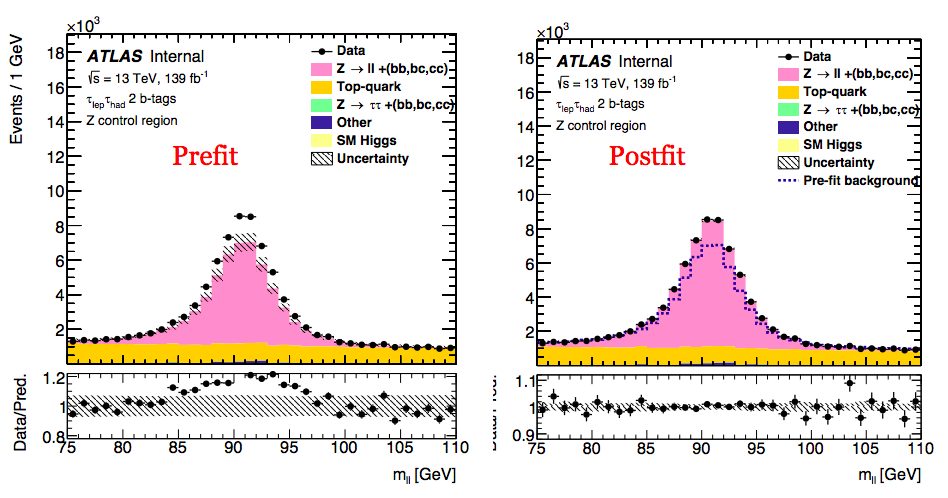
\includegraphics[width=0.95\textwidth]{figures/auxiliary/ZHF_mll.png}}
% \subfigure[]{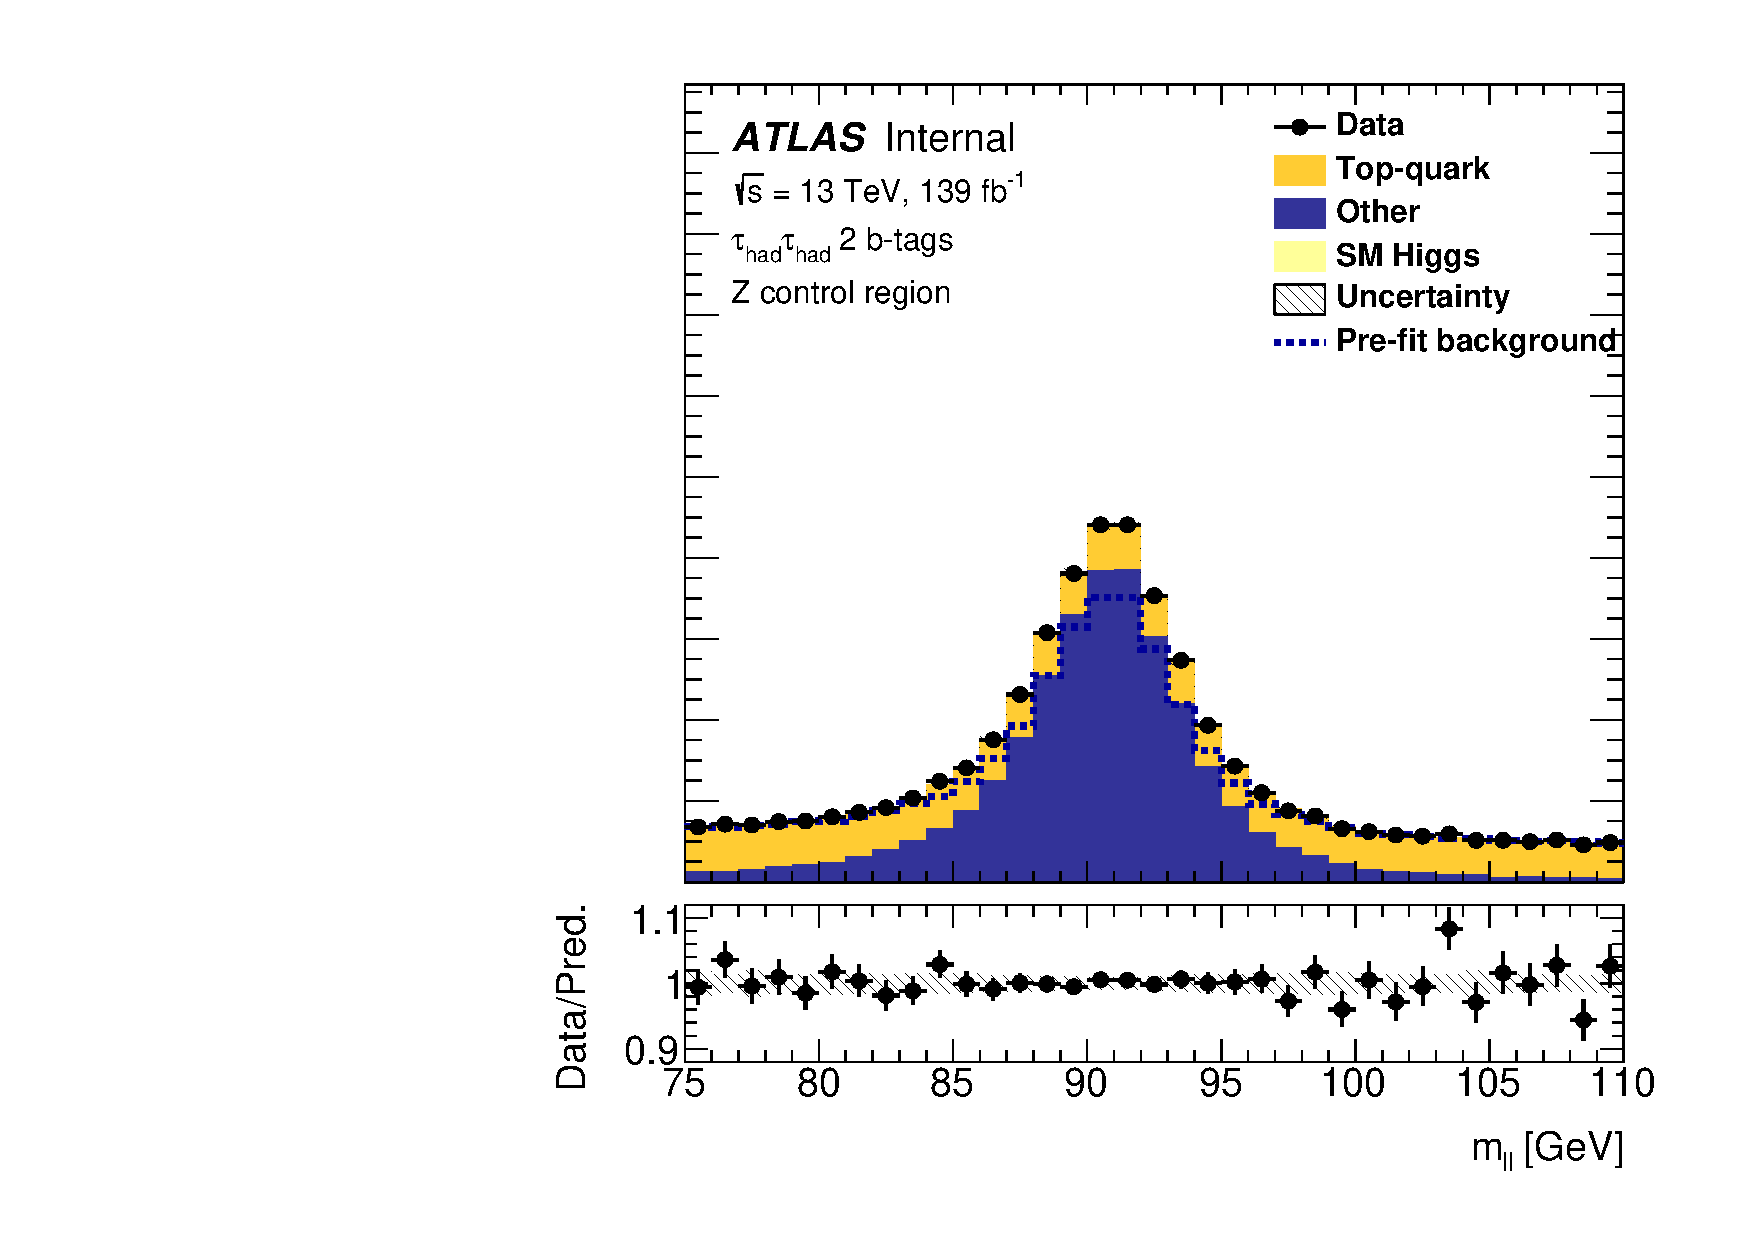
\includegraphics[width=0.50\textwidth]{figures/PostfitPlots/Region_BMin0_incJet1_Y2015_DZllbbCR_T2_L2_distmLL_J2_GlobalFit_conditionnal_mu0.pdf}}
% %%% \caption{(a) Pre-fit background and data and (b) post-fit background and data $m_{\ell\ell}$ distributions in the $Z+\text{HF}$ control region. In (b), the normalisation and shape of the backgrounds and the uncertainty on the total background are shown as determined from the likelihood fit to data in the non-resonant $HH$ search. The uncertainty band includes statistical and systematics uncertainties on the total background. \TODO{change to up-to-date plots.}}
% \caption{Post-fit background and data $m_{\ell\ell}$ distributions in the $Z+\text{HF}$ control region. The normalisation and shape of the backgrounds and the uncertainty on the total background are shown as determined from the likelihood fit to data in the non-resonant $HH$ search. The uncertainty band includes statistical and systematics uncertainties on the total background. The dashed histogram shows the total pre-fit background.}
% \label{fig:zcr}
% \end{figure}
